\documentclass[tikz,border=12pt]{standalone}
% Shared visual language for standalone EMT block diagrams.
\usepackage{amsmath}
\usetikzlibrary{arrows.meta,backgrounds,calc,fit,positioning}

\tikzset{
    emt diagram/.style = {>={Stealth[length=2.4mm]}},
    line/.style        = {semithick, rounded corners=6pt},
    block/.style       = {draw, semithick, fill=white,
                          minimum height=1cm, minimum width=2.3cm},
    hblock/.style      = {block, minimum width=2.24cm, minimum height=1.3cm},
    vblock/.style      = {block, minimum width=1.3cm, minimum height=2.24cm},
    sum/.style         = {draw, semithick, fill=white, circle,
                          inner sep=2.6pt},
    signal/.style      = {circle, fill, inner sep=1.4pt,
                          label distance=3pt},
    sig/.style         = {font=\small},
    pm/.style          = {font=\scriptsize},
    wire jump/.style   = {line,
                          preaction={draw=white, line width=3pt,
                                     line cap=round}},
    enclosure/.style   = {draw, dashed, semithick, rounded corners=4pt},
    operator enclosure/.style = {enclosure, inner xsep=7mm, inner ysep=6mm}
}


\begin{document}
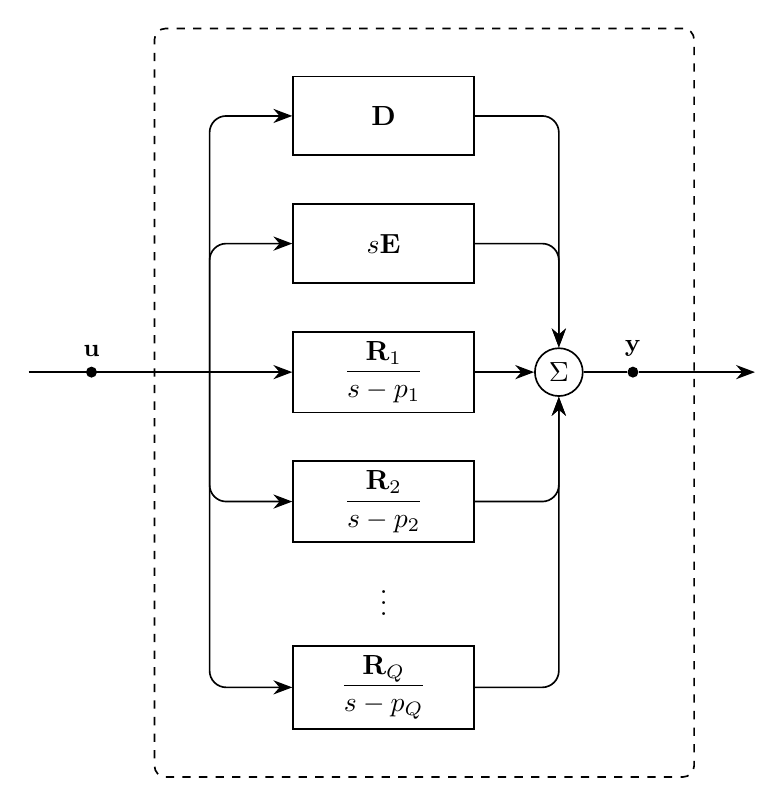
\begin{tikzpicture}[emt diagram]

% Parallel branches
\node[block] (R1) {$\dfrac{\mathbf{R}_1}{s - p_1}$};
\node[block, above=0.6cm of R1] (E) {$s\mathbf{E}$};
\node[block, above=0.6cm of E] (D) {$\mathbf{D}$};
\node[block, below=0.6cm of R1] (R2) {$\dfrac{\mathbf{R}_2}{s - p_2}$};
\node[block, below=1.3cm of R2] (RQ) {$\dfrac{\mathbf{R}_Q}{s - p_Q}$};
\node at ($(R2)!0.5!(RQ)$) {$\vdots$};

% Fan-out from a single internal point
\coordinate (split) at ($(R1.west)+(-1.05, 0)$);
\draw[->, line] (split) -- (R1.west);
\foreach \b in {D, E, R2, RQ}
    \draw[->, line] (split) |- (\b.west);

% Fan-in to summation
\node[sum, right=0.75cm of R1] (S) {$\Sigma$};
\draw[->, line] (R1.east) -- (S);
\foreach \b/\a in {D/north, E/north, R2/south, RQ/south}
    \draw[->, line] (\b.east) -| (S.\a);

% Input node (owned externally)
\node[signal, label={[sig]above:$\mathbf{u}$}] (uin)
    at ($(split)+(-1.5, 0)$) {};
\draw[line] ($(uin)+(-0.8, 0)$) -- (split);

% Output node (owned by this model) with port arrow out
\node[signal, label={[sig]above:$\mathbf{y}$}, right=0.55cm of S]
    (yout) {};
\draw[line] (S.east) -- (yout);
\draw[->, line] (yout) -- ++(1.55, 0);

% Model enclosure: fixed padding around model-owned paths and output variable
\begin{scope}[on background layer]
    \node[operator enclosure, fit=(split)(D)(E)(R1)(R2)(RQ)(S)(yout)] {};
\end{scope}

\end{tikzpicture}
\end{document}
